\documentclass[journal]{IEEEtran}
\usepackage[T1]{fontenc}
\usepackage{lmodern}
\usepackage{amsmath}
\usepackage{graphicx}
\usepackage{booktabs}
\usepackage{siunitx}
\usepackage{tikz}
\usetikzlibrary{positioning,arrows.meta}
\usepackage[hidelinks]{hyperref}
\sisetup{group-separator={,},group-minimum-digits=4}

\markboth{Working Draft: Feedback Requested}{Starkey: A Danger-Field PPO Controller for Dodge}

\begin{document}

\title{A Danger-Field PPO Controller for the Dodge Arcade Game: Hard-Difficulty
Evaluation, Decision Frequency, and Where Games End}

\author{Lucas~Starkey%
\thanks{This is a working draft written to solicit feedback. Results are
exploratory, come from a single training lineage, and have not been peer
reviewed.}}

\maketitle

\begin{abstract}
We report the current state of a reinforcement-learning agent for Dodge, a
small score-driven arcade game whose hazards intensify as the player scores.
The cartridge's own Lua source runs headlessly under LuaJIT inside a partial
PICO-8 runtime written in Python. The policy, VelocityFlow~v2, is a
111k-parameter convolutional network whose only output is a time-sliced danger
field over the arena; a fixed controller reads that field along the simulated
path of each of the nine actions, so the logits are path danger and nothing
between field and action is learned. After 21,051 PPO updates (43.2M
decisions), the best checkpoint survives a mean of 3,922 alive frames
(65~seconds) on the hardest setting, with a worst-quarter mean of 1,180, on
512 fresh seeds. It beats an earlier checkpoint on the same seeds by
623~frames (95\% interval $+223$ to $+975$). Evaluating it with a decision every
fourth frame instead of every frame halves survival ($-1{,}805$ frames), the
reverse of a recent report's ``control-frequency surprise'' and consistent
with our checkpoint having been trained on per-frame decisions. Observation-only
death telemetry shows that the anti-camping guard never fires for this policy,
that 74\% of deaths occur while a pattern is active (in 44\% of frames), and
that 69\% of enemy-contact deaths happen during patterns. Replaying the 310
deaths inside static patterns shows two recurring shapes: running along a wall
into a bar, and circling in the open centre until an enemy closes in. We
describe the game, model, and protocol, report these results with their
limits, and pose specific questions.
\end{abstract}

\begin{IEEEkeywords}
reinforcement learning, proximal policy optimization, potential fields,
convolutional networks, action repeat, evaluation methodology, arcade games
\end{IEEEkeywords}

\section{Introduction}
\IEEEPARstart{D}{odge} is a short arcade game in which the player steers a
square around a small arena, avoids moving enemies and large rectangular
hazards, and collects pickups that raise the score. Scoring makes the game
faster and more dangerous, so the objective that looks natural, a high score,
conflicts with the one that keeps the player alive.

This draft follows the evaluation protocol of a recent working draft on the
same game by Turner~\cite{turner}, which trained an entity-transformer teacher
on a Rust port, so that the two efforts can be compared on like terms: alive
frames, quarter means, sampled versus argmax actions, one- versus four-frame
decisions, and instrumented death telemetry. The two projects differ in
almost everything else: simulator, observation, architecture, reward,
difficulty, and training history. Cross-paper comparisons of levels are
therefore indicative only (Section~\ref{sec:limits}).

We do not present a finished or competitive agent. The contributions we think
are of interest are:
\begin{enumerate}
\item A field-only policy: a convolutional network that predicts danger per
  arena cell at six future times, read by a fixed path-sampling controller, so
  that the network never outputs an action directly (Section~\ref{sec:model}).
\item A paired, 512-seed evaluation of the best checkpoint on the hardest
  setting, with bootstrap intervals and an earlier checkpoint and two
  baselines on the same seeds (Section~\ref{sec:headline}).
\item A decision-frequency result that runs opposite to~\cite{turner}:
  coarser decisions halve survival for a policy trained at one decision per
  frame (Section~\ref{sec:k}).
\item Death telemetry: the anti-camping guard is absent from this policy's
  deaths, while patterns, and enemies during patterns, account for most of
  them; replayed paths into the deadliest static patterns
  (Sections~\ref{sec:where}--\ref{sec:paths}).
\end{enumerate}
Section~\ref{sec:questions} lists the questions on which we most want input.

\section{The Game}
Dodge is a PICO-8 cartridge by Artridge~\cite{artridge}. The playfield is a
$128\times128$ pixel square updated at 60\,Hz. The player moves in eight
directions or stays still. Movement has inertia: each frame velocity is
multiplied by 0.8 and each held direction adds 0.5, so the effect of an
action depends on current motion.

\emph{Hazards.} Enemies enter the arena, home on the player, grow, and collide
with one another. Kamikaze enemies leave a growing explosion. Pattern events
add large rectangles that are telegraphed before becoming lethal: static
patterns, whose rectangles hold or morph in place, and moving patterns, which
sweep across the field. Some pattern geometry extends past the visible screen.

\emph{Pickups and score.} Pickups explode nearby enemies, freeze the game, or
shrink the player; score rises when enemies die and when pickups are
collected. Game speed, enemy spawn timing, and the pool of eligible patterns
depend on score.

\emph{Anti-camping guard.} If the player stays inside a small central
region for more than 50 consecutive frames, the cartridge
routine \texttt{fyou} spawns an enemy at every spawn point.

\emph{Death.} A game ends on the first lethal contact. We record its class:
normal enemy, kamikaze (body or explosion), static-pattern rectangle, or
moving-pattern rectangle.

\section{Environment and Observations}
\emph{Simulator.} The game is not ported. A Python runtime implements the
subset of the PICO-8 API the cartridge uses and executes the cartridge's own
Lua under LuaJIT via \texttt{lupa}; a null backend skips rendering. Training
controls (enemy-type switches, spawn-rate scaling, event counters) are layered
over the unmodified cartridge functions rather than edited into its source.
Rounds start directly in gameplay with the cartridge's keyboard movement
model. All runs here use the hard setting (cartridge difficulty~3) with
patterns, powerups, and both enemy types on at 100\% spawn rate.

\emph{Units.} A frame is one 1/60\,s update. A decision is one policy action,
held for $K$ frames. The current training configuration uses $K=1$; the
discount and GAE decay are defined per decision.

\emph{Observation.} Each decision sees a single frame (Table~\ref{tab:io}):
the player's position and velocity, and a $32\times32$ grid of 4-pixel cells,
each holding an entity category (eight types: three enemy kinds, three
pickups, a pattern warning, a lethal pattern rectangle) and that entity's
velocity in two planes. Motion is read from the game, not inferred from frame
differences, because everything moves less than one cell per decision. When
two entities share a cell the more dangerous one is kept. Warnings are encoded
for exactly as long as the cartridge draws them. The agent never sees seeds,
hidden timers, or future pattern schedules.

\emph{Reward.} Per frame survived, $+0.02$; plus the score change, where score
from enemies destroying one another (0.5 per enemy, not caused by the agent)
is weighted 0.05 and all other score 1.0; and $-2$ on death. A frame cap
while the player is alive is a truncation and bootstraps; death is a
termination and does not~\cite{pardo}.

\begin{table}[t]
\caption{Policy inputs and outputs.}
\label{tab:io}
\centering
\begin{tabular}{@{}ll@{}}
\toprule
Item & Content \\
\midrule
Player & 4 floats: $p_x, p_y, \dot p_x, \dot p_y$ \\
Grid & $32\times32$ cells: category $\in\{0..8\}$, $v_x$, $v_y$ \\
Observation & 3,076 floats, one frame, no stack \\
Field output & $6\times32\times32$ danger, slices at 4--108 frames \\
Actions & 9 (neutral, 4 cardinal, 4 diagonal) \\
Value output & 1 scalar \\
\bottomrule
\end{tabular}
\end{table}

\section{Model and Training}\label{sec:model}
\emph{Architecture.} VelocityFlow~v2 (Fig.~\ref{fig:arch}) is fully
convolutional up to its output. A trunk of four $3\times3$ convolutions
(32--64 channels, one dilated) maps the one-hot grid, velocity planes, and
player channels to 32 feature maps; its three heavy layers run at
$16\times16$ and are interpolated back to $32\times32$. A context branch pools
the trunk to $4\times4$, convolves, and is bilinearly upsampled and
concatenated, so every cell sees an arena-wide summary. A $1\times1$ head
emits six danger fields, one per future time
$t\in\{4,12,24,48,72,108\}$ frames.

\emph{Controller.} For each action, the cartridge's movement model gives the
player's offset at each $t$ (from rest). The controller samples field slice
$t$ at the player's position plus that offset, weights the six samples by
$0.985^t$, and negates the sum. The nine path dangers are standardised across
actions and multiplied by a learned temperature to give the logits; there is
no policy head. The temperature, initialised at 0.5, had grown to 6.4 in the
best checkpoint.

\emph{Critic.} The value head sees the trunk's channel means, an
$8\times4\times4$ coarse arena map, and the player inputs, through a 64-unit
MLP. All activations are LeakyReLU. The model has 111,424 parameters.

\emph{PPO.} We use Stable-Baselines3~\cite{sb3} PPO~\cite{ppo} with
GAE~\cite{gae} (Table~\ref{tab:ppo}). Each update collects 256 decisions from
each of eight environments and runs four epochs of 256-sample minibatches
with a KL early stop. Training ran in a dashboard that allowed game settings
and reward weights to be changed between updates; checkpoints do not record
which settings were in force when, so the training curriculum is not
reconstructible from the checkpoints alone.

\begin{figure}[t]
\centering
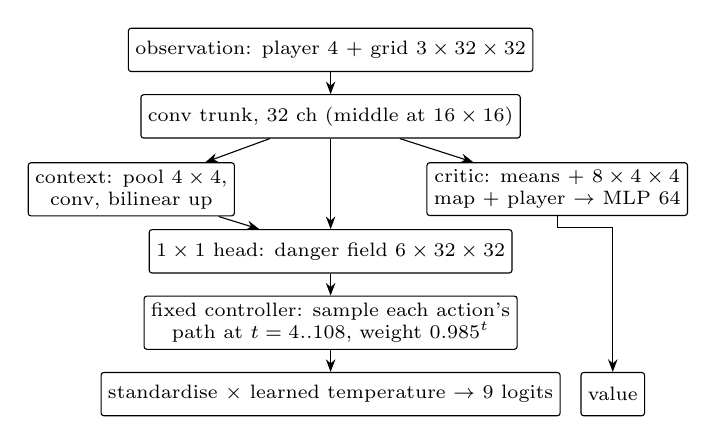
\begin{tikzpicture}[
  box/.style={draw, rounded corners=1pt, align=center, font=\scriptsize,
              inner sep=2.5pt, minimum height=0.55cm},
  ar/.style={-{Stealth[length=1.6mm]}, thin}]
\node[box] (obs) {observation: player 4 + grid $3\times32\times32$};
\node[box, below=0.28cm of obs] (trunk) {conv trunk, 32 ch (middle at $16\times16$)};
\node[box, below left=0.3cm and -1.2cm of trunk] (ctx) {context: pool $4\times4$,\\conv, bilinear up};
\node[box, below right=0.3cm and -1.2cm of trunk] (val) {critic: means + $8\times4\times4$\\map + player $\to$ MLP 64};
\node[box, below=1.15cm of trunk] (field) {$1\times1$ head: danger field $6\times32\times32$};
\node[box, below=0.28cm of field] (ctrl) {fixed controller: sample each action's\\path at $t=4..108$, weight $0.985^t$};
\node[box, below=0.28cm of ctrl] (logit) {standardise $\times$ learned temperature $\to$ 9 logits};
\node[box, right=0.25cm of logit] (v) {value};
\draw[ar] (obs) -- (trunk);
\draw[ar] (trunk) -- (ctx);
\draw[ar] (trunk) -- (val);
\draw[ar] (ctx) -- (field);
\draw[ar] (trunk) -- (field);
\draw[ar] (field) -- (ctrl);
\draw[ar] (ctrl) -- (logit);
\draw[ar] (val.south) -- ++(0,-0.15) -| (v.north);
\end{tikzpicture}
\caption{VelocityFlow~v2. The network's only policy output is the danger field;
actions are chosen by reading it along simulated paths.}
\label{fig:arch}
\end{figure}

\begin{table}[t]
\caption{PPO settings (all three VelocityFlow~v2 checkpoints).}
\label{tab:ppo}
\centering
\begin{tabular}{@{}ll@{}}
\toprule
Setting & Value \\
\midrule
Discount $\gamma$, GAE $\lambda$ & 0.99, 0.95 \\
Clip, entropy coef., value coef. & 0.2, 0.01, 1.0 \\
Epochs, minibatch, grad-norm clip & 4, 256, 0.5 \\
Rollout & 8 envs $\times$ 256 decisions \\
Target KL (epoch early stop) & 0.02 \\
Learning rate & $3\times10^{-4}$, constant \\
\bottomrule
\end{tabular}
\end{table}

\section{Evaluation Protocol}\label{sec:protocol}
All numbers are alive frames at 60\,Hz on the hard setting with patterns and
powerups on and an 18,000-frame cap, unless stated. As in~\cite{turner} we
report Worst and Best (single games), Median, Mean, and two quarter means: Q1
is the mean of the worst 25\% of games and Q4 the mean of the best 25\%; Q1 is
not the 25th percentile. We treat the lower tail as primary.

Every condition plays the same 512 seeds (256 for the earlier checkpoint and
random baseline, 128 for the heuristic), a contiguous block starting at 1,000,000;
training draws 31-bit seeds at random, so overlap is improbable but not
excluded. Differences are paired by seed
and bootstrapped by seed (2,000 resamples); single-condition intervals use
4,000 resamples for the mean and 1,000 for Q1. Argmax evaluation chooses the most likely action; sampled evaluation
draws from the policy. The evaluator runs up to 64 games in lockstep with
batched GPU inference. In a spot check, a batched GPU game matched an
unbatched CPU run of the same seed in frame, cause, and score, and the telemetry hooks wrap cartridge
functions without touching the random-number generator.

The best checkpoint was evaluated as tracked in the repository
(\texttt{velocity-flow-v2-latest.zip}, SHA-256 prefix
\texttt{71e3733d91a56f94}). No evaluation result was used to choose a
training setting; the only selection made on this cohort is the comparison
of two checkpoints in Section~\ref{sec:headline}.

\section{Results}

\subsection{The best checkpoint}\label{sec:headline}
Table~\ref{tab:main} gives the headline numbers. With a decision every frame
and argmax actions, the best checkpoint survives a mean of 3,922 frames
(95\% interval 3,707--4,138) and a median of 3,600; its worst quarter averages
1,180 (1,047--1,328). 89\% of games pass 1,000 frames, 46\% pass 4,000 and 6\%
pass 8,000 (Fig.~\ref{fig:survival}). No game reached the cap; the longest
lasted 15,235 frames (17,732 with sampled actions).

On the same 256 seeds, the earlier \texttt{can-reach-100} checkpoint (5,691
updates) averages 3,208. The later checkpoint is ahead by 623 frames in mean
($+223$ to $+975$) and 431 in Q1 ($+175$ to $+674$), so the additional 15,360
updates helped, the lower tail included. A uniformly random policy survives
196 frames. The repository's hand-written gradient-field controller survives
126: on this setting it idles at the spawn point, triggers the anti-camping
guard at frame~51, and dies near frame~119 in almost every game. It is
therefore not a meaningful upper reference here, unlike the 6,115-frame
heuristic in~\cite{turner}.

\begin{table}[t]
\caption{Survival on fresh seeds, hard setting, alive frames.
1f/4f: one/four frames per decision.}
\label{tab:main}
\centering
\setlength{\tabcolsep}{3.2pt}
\resizebox{\columnwidth}{!}{%
\begin{tabular}{@{}llrrrrrrr@{}}
\toprule
Policy & Mode & $n$ & Worst & Q1 & Median & Mean & Q4 & Best \\
\midrule
v2-latest & 1f argmax  & 512 & 453 & 1,180 & 3,600 & 3,922 & 7,262 & 15,235 \\
v2-latest & 1f sampled & 512 & 176 & 1,106 & 3,757 & 3,854 & 7,034 & 17,732 \\
v2-latest & 4f argmax  & 512 & 235 & 601 & 1,790 & 2,118 & 4,158 & 8,668 \\
v2-latest & 4f sampled & 512 & 127 & 577 & 1,582 & 1,865 & 3,708 & 7,830 \\
\midrule
can-reach-100 & 1f argmax & 256 & 213 & 824 & 3,292 & 3,208 & 5,747 & 9,709 \\
random & 1f & 256 & 72 & 110 & 188 & 196 & 302 & 541 \\
gradient field & 1f & 128 & 119 & 119 & 119 & 126 & 145 & 259 \\
\bottomrule
\end{tabular}}
\end{table}

\begin{figure}[t]
\centering
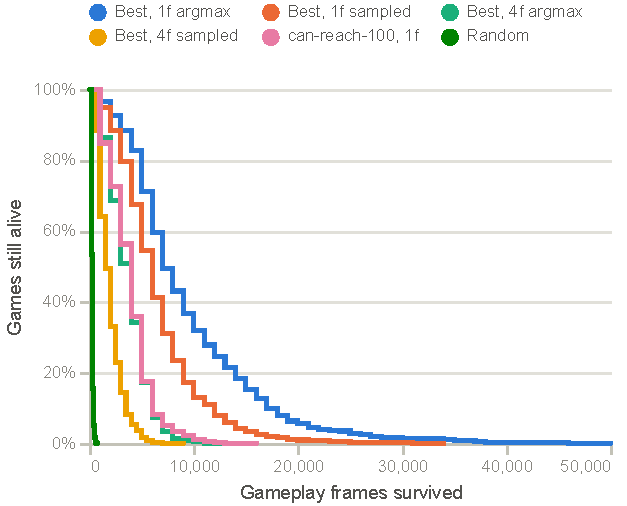
\includegraphics[width=\columnwidth]{fig_survival.pdf}
\caption{Share of games still alive at each 1,000-frame milestone
(\texttt{velocity-flow-v2-latest}, 512 fresh seeds per line; baselines on
their own seed counts).}
\label{fig:survival}
\end{figure}

\subsection{Decision frequency}\label{sec:k}
Turner~\cite{turner} found that a policy trained with $K=4$ more than doubled
its worst-quarter survival when evaluated at $K=1$ with frozen weights. We ran
the same $2\times2$ design, $K\in\{1,4\}$ by action mode, on our checkpoint,
whose current training configuration is $K=1$ (Fig.~\ref{fig:kgrid}). The
effect is of similar size and opposite sign. Moving to four-frame decisions
lowered the mean by 1,805 frames under argmax ($-2{,}054$ to $-1{,}555$) and
1,989 under sampling, and Q1 by 578 ($-731$ to $-430$) and 529. Under $K=4$,
29\% of games end before frame 1,000, against 11\% at $K=1$.

Argmax and sampling are indistinguishable at $K=1$ (mean $+68$, $-242$ to
$+365$; Q1 $+74$, $-139$ to $+281$). At $K=4$, argmax is ahead in mean
($+253$, $+80$ to $+415$) but not in Q1 ($+24$, $-52$ to $+105$).

Read together with~\cite{turner}, the simplest account is that a policy does
best at the decision rate it was trained for, and that for both policies that
rate leaves the agent better off when it is one frame. One detail is specific
to our controller: its action-path offsets were computed for an action held
four frames, and that table is stored in every checkpoint and was not
regenerated when training moved to $K=1$. The policy therefore scores its nine
actions as if each were held four frames, while executing each for one.

\begin{figure}[t]
\centering
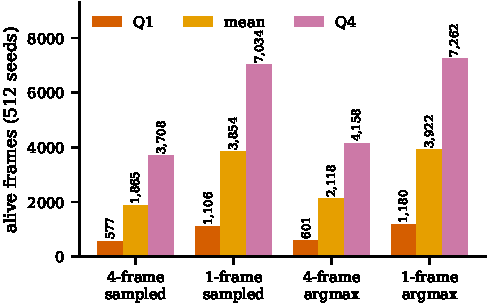
\includegraphics[width=\columnwidth]{fig_k_grid.pdf}
\caption{One frozen checkpoint, four versus one frame per decision, sampled
and argmax, on the same 512 fresh seeds. Q1 is the mean of the worst 25\% of
games.}
\label{fig:kgrid}
\end{figure}

\subsection{Where games end}\label{sec:where}
Fig.~\ref{fig:causes} splits the first lethal contact by the window in which
the game ended. At $K=1$, normal enemies account for 59--77\% of deaths in
every window and 71\% overall; kamikazes 10\%, static-pattern rectangles
15\%, moving-pattern rectangles 3\%. Rectangles matter most early: they are
27\% of deaths before frame 1,000 and 28\% between 1,000 and 2,000, falling to
13--19\% later. At $K=4$, deaths shift heavily toward the first 2,000 frames
(56\% of games end there, against 27\% at $K=1$) and toward normal enemies.

\begin{figure*}[t]
\centering
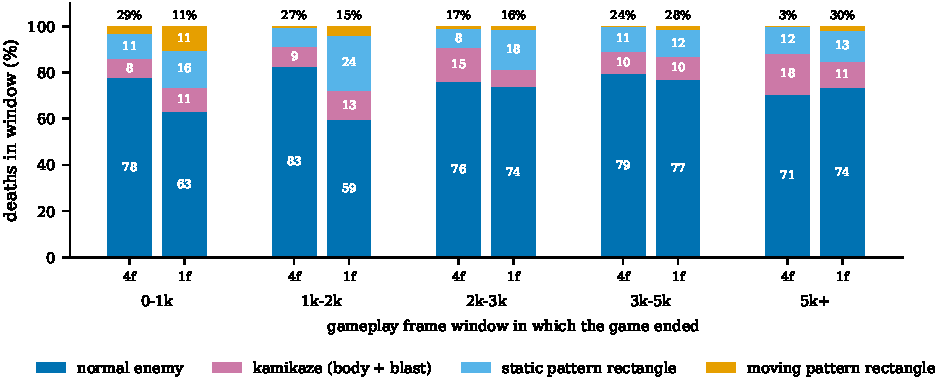
\includegraphics[width=\textwidth]{fig_causes.pdf}
\caption{First lethal contact by the window in which the game ended,
\texttt{velocity-flow-v2-latest}, argmax, 512 fresh games per setting (4f:
$K=4$; 1f: $K=1$). The percentage above each bar is that window's share of
all games.}
\label{fig:causes}
\end{figure*}

\subsection{Death telemetry: guard, patterns, and enemies}\label{sec:telemetry}
We added an observation-only recorder in Lua: it wraps the cartridge's
\texttt{collide}, \texttt{die}, \texttt{fyou}, \texttt{addenemy} and
\texttt{updatepatterns} functions, logs every anti-camping trigger and the
enemies it spawns, every pattern encounter by identifier, and at the first
lethal contact the killer's class and the active pattern. It consumes no
random numbers and does not touch reward or observation; a recorded game
reproduces the unrecorded game frame for frame.

\emph{The guard is not involved.} The anti-camping guard fired in none of the
2,048 games of the best checkpoint, under any setting, so none of its deaths
follow a trigger. The earlier \texttt{can-reach-100} checkpoint triggered it in
97.7\% of games, although its spawns killed the player in only 2 of 203
enemy-contact deaths. Somewhere between the two checkpoints the policy
stopped lingering in the centre.

\emph{Patterns are where games end.} A pattern is active in 44\% of the frames
the best checkpoint lives at $K=1$ but in 74\% of its deaths: 4.35 deaths per
10,000 frames with a pattern active against 1.16 without, a ratio of 3.8. At
$K=4$ the rates are 7.41 and 2.78 (ratio 2.7). Of 512 deaths at $K=1$, 310
happen during static patterns, 71 during moving patterns, and 131 with no
pattern active. The ratio is smaller than the 14--27$\times$ reported
in~\cite{turner}; we have not established why.

\emph{The policy loses to enemies while patterns are active.} 69\% of
enemy-contact deaths at $K=1$ occur during a pattern, and only 94 of the 381
deaths during a pattern are rectangle contact. Lethality is concentrated but
not in a short list (Fig.~\ref{fig:patterns}). Among patterns met at least 30
times, pattern 28 ends 34\% of its 144 encounters in death, pattern 21 32\%,
patterns 17 and 18 26\%. Patterns 18 and 28 are each the active pattern in 13
of the 57 deaths before frame 1,000. At $K=4$ the same two patterns are far
deadlier (18: 57\%, 28: 49\%); all but three of the frequently met patterns
are more lethal at $K=4$, and those three differ by at most three points.

\begin{figure*}[t]
\centering
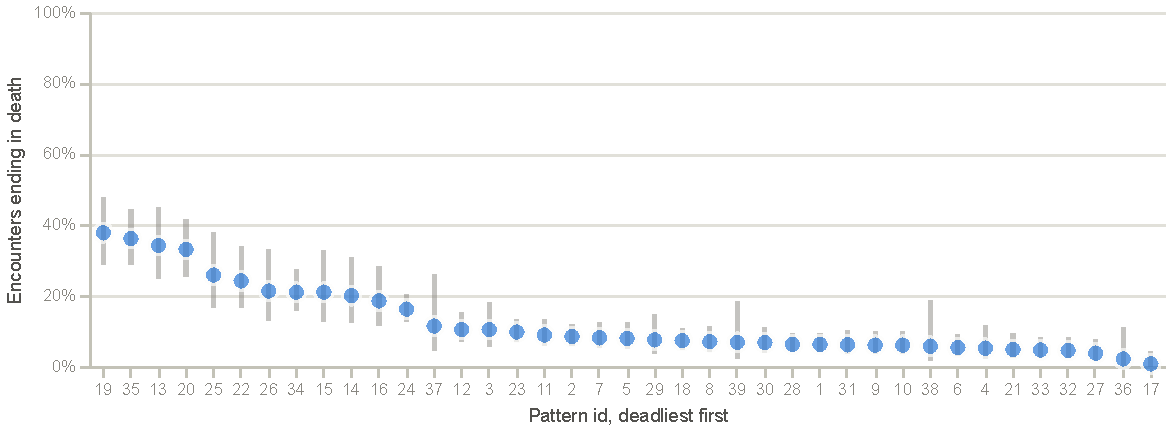
\includegraphics[width=\textwidth]{fig_patterns.pdf}
\caption{Share of encounters with each pattern during which the player died,
for patterns met at least 30 times at $K=1$ (filled, with 95\% Wilson
intervals), and the same at $K=4$ (hollow). Score-gated patterns appear only
later in a game, so cross-identifier comparisons mix lethality with exposure
at higher score.}
\label{fig:patterns}
\end{figure*}

\subsection{Paths into the deadliest static patterns}\label{sec:paths}
We replayed all 310 games that ended during a static pattern ($K=1$, argmax)
with a per-frame recorder of the player's position, the lethal rectangles at
the death frame, and the killer's position. 309 replays ended on the same
frame with the same cause as the original run; one (seed 1,000,395) diverged
late, ending 254 frames earlier on the same pattern and cause, which we
attribute to floating-point differences between batch compositions in GPU
inference. Fig.~\ref{fig:paths} shows the last 60 frames before death in the
four static patterns with the most deaths.

Two shapes recur. In pattern 28, a frame of four bars, deaths to a rectangle
(17 of 49) run down the left wall into the side bar, while deaths to enemies
circle in the open centre until an enemy arrives. In pattern 18, a ring of
wall bars with gaps at the midpoints (35 deaths, 30 to enemies), paths wander
in the open interior and end at an enemy, not at a wall. Patterns 1 and 21
(18 deaths each) show the same mixture at lower density. These shapes
resemble the wall-running and circling failures reported in~\cite{turner},
which may mean they are properties of the game's layouts rather than of
either architecture.

These are associations at the death frame. They have no counterfactual: we
cannot say the policy ``should'' have turned away. Distinguishing a perception
failure from a planning failure needs counterfactual branching: restore a
state about 60 frames before death and vary the actions.

\begin{figure*}[t]
\centering
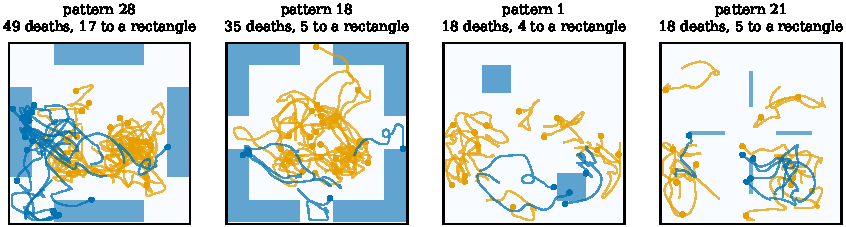
\includegraphics[width=\textwidth]{fig_paths.pdf}
\caption{Last 60 frames before death inside the four static patterns with the
most deaths (\texttt{velocity-flow-v2-latest}, $K=1$, argmax; up to 45 paths
each, first by seed). Blue: died to the rectangle; orange: died to an enemy;
dots mark the death position. Shading is the share of these deaths at which
each pixel lay inside a lethal rectangle; static rectangles move within a
pattern, so no single layout is representative.}
\label{fig:paths}
\end{figure*}

\section{Limitations}\label{sec:limits}
\emph{One lineage.} All checkpoints descend from one training lineage; the
comparison between checkpoints is between two points of it, not between
training replicas, and evaluation seeds do not substitute for
those~\cite{henderson,agarwal}. \emph{Unrecorded training history.} The
decision interval, difficulty, reward weights and lives in force during
training were changed interactively and are not stored with the checkpoints;
the reward described is the current configuration. \emph{One cohort.} A
single 512-seed cohort served both the checkpoint comparison and the
reported levels; there was no separate confirmation cohort. \emph{Replay
determinism.} Batched GPU inference reproduced 309 of 310 replays exactly.
\emph{Baselines.} Neither baseline calibrates the upper end: the gradient-field
heuristic fails on this setting for a reason unrelated to dodging. \emph{Cross-paper
comparison.} Turner~\cite{turner} reports normal difficulty on a Rust port with
a different reward and observation; we report hard difficulty on the original
Lua. Levels are not directly comparable. \emph{No explanation.} The telemetry
is descriptive and has no counterfactuals.

\section{Questions for Practitioners}\label{sec:questions}
We would especially value opinions on the following.
\begin{enumerate}
\item \emph{Path offsets.} Our controller scores actions with paths for a
  four-frame hold while executing one-frame decisions. Should the offsets
  match the executed interval, or is a longer assumed hold a useful bias
  toward committed motion? How would you test that without retraining from
  scratch?
\item \emph{Pursuit.} A scalar field over positions cannot express ``step
  aside because it is chasing you''; enemies during patterns are our largest
  killer. Would you condition the field on the candidate action, add an
  explicit pursuit channel, or move to a learned head over field features?
\item \emph{Lower tail.} Q1 is 30\% of the mean. Is the next gain more likely
  from representation (short-term memory), objective (score in the reward),
  or exposure (more late-game, high-score patterns in training)?
\item \emph{Selection.} Given one lineage and hours per run, what is the
  minimum protocol (cohort sizes, confirmation splits, training seeds) you
  would accept for declaring a checkpoint best?
\item \emph{Baseline.} What hand-written controller would you use as an upper
  reference on the hard setting, given that a pure danger-gradient follower
  is defeated by the anti-camping guard?
\end{enumerate}

\section{Conclusion}
A field-only PPO controller for Dodge reaches a mean of 3,922 alive frames
and a worst-quarter mean of 1,180 on the hardest setting, and more training
measurably helped. Decision frequency again matters more than many training
updates, but in the direction of the rate the policy was trained for. Death
telemetry points at enemies that close in while patterns are active, not at
the rectangles themselves and not at the anti-camping guard. We offer the
setup and numbers as an honest, partly negative record and invite critique.

\section*{Availability}
The toolchain (cartridge extractor, PICO-8 runtime, environment, training
dashboard) is at \url{https://github.com/LaunchSpark/DodgeAI}. It contains no
game content; the cartridge must be obtained from the original
release~\cite{artridge}. Selected checkpoints are tracked in the repository.

\section*{Acknowledgment}
Experiments and this draft were prepared with an AI coding agent (Claude)
under human direction; the author reviewed the claims and takes
responsibility for them. The evaluation protocol follows~\cite{turner}. The
original Dodge game and its art are by Artridge.

\begin{thebibliography}{10}
\bibitem{turner}
T.~Turner, ``An entity-transformer {PPO} teacher for the {Dodge} arcade game:
Evaluation pitfalls, a control-frequency surprise, and open questions,''
working draft, 2026.
\bibitem{artridge}
Artridge, ``Dodge,'' PICO-8 game, Lexaloffle BBS.
\url{https://www.lexaloffle.com/bbs/?pid=66443}
\bibitem{pardo}
F.~Pardo, A.~Tavakoli, V.~Levdik, and P.~Kormushev, ``Time limits in
reinforcement learning,'' in \emph{Proc. Int. Conf. Machine Learning (ICML)},
2018.
\bibitem{sb3}
A.~Raffin, A.~Hill, A.~Gleave, A.~Kanervisto, M.~Ernestus, and N.~Dormann,
``Stable-Baselines3: Reliable reinforcement learning implementations,''
\emph{J. Machine Learning Research}, vol.~22, no.~268, pp.~1--8, 2021.
\bibitem{ppo}
J.~Schulman, F.~Wolski, P.~Dhariwal, A.~Radford, and O.~Klimov, ``Proximal
policy optimization algorithms,'' arXiv:1707.06347, 2017.
\bibitem{gae}
J.~Schulman, P.~Moritz, S.~Levine, M.~Jordan, and P.~Abbeel,
``High-dimensional continuous control using generalized advantage
estimation,'' in \emph{Proc. Int. Conf. Learning Representations (ICLR)},
2016.
\bibitem{henderson}
P.~Henderson, R.~Islam, P.~Bachman, J.~Pineau, D.~Precup, and D.~Meger, ``Deep
reinforcement learning that matters,'' in \emph{Proc. AAAI Conf. Artificial
Intelligence}, 2018.
\bibitem{agarwal}
R.~Agarwal, M.~Schwarzer, P.~S.~Castro, A.~Courville, and M.~G.~Bellemare,
``Deep reinforcement learning at the edge of the statistical precipice,'' in
\emph{Advances in Neural Information Processing Systems (NeurIPS)}, 2021.
\end{thebibliography}

\end{document}
